\section{Component Interface}
\label{sec:impl_component_interface}

The \texttt{CoSimComponent} base class implements the common runtime contract for all simulation components in \syssimx{}.
It realizes the component abstraction introduced in Section~\ref{sec:architecture_cosimcomponent} and builds on the port system of Section~\ref{sec:impl_port_system}.
The class centralizes lifecycle control, port-state management, history recording, and common structural and hybrid metadata.
Backend wrappers therefore only implement the model-specific operations.

%%%%%%%%%%%%%%%%%%%%%%%%%%%%%%%%%%%%%%%%%%%%%%%%%%%%%%
\subsection{Design}

\texttt{CoSimComponent} is implemented as an abstract base class that follows the template method pattern~\cite{gamma_design_1995}.
The public lifecycle methods define a fixed execution skeleton.
Primitive operations provide the mandatory subclass-specific behavior.
Hook operations extend the contract for features such as state transfer, rollback, zero-step output evaluation, and event handling.
Table~\ref{tab:component_methods} summarizes this organization.

%
\begin{table}[!htbp]
  \centering
  \small
  \caption{Role-based classification of the main \texttt{CoSimComponent} methods.
  Template methods define the public lifecycle.
  Primitive operations are implemented by each subclass.
  Hook operations provide optional extension points.}
  \label{tab:component_methods}
  \begin{tabular}{llp{5.8cm}}
    \toprule
    \textbf{Method} & \textbf{Contract} & \textbf{Purpose} \\
    \midrule
    \texttt{initialize(t0)}                              & Template  & Component lifecycle startup \\
    \texttt{do\_step(t, dt)}                             & Template  & Macro time step \\
    \texttt{handle\_event(event\_names, t)}              & Template  & Event handling and output refresh \\
    \midrule
    \texttt{\_initialize\_component(t0)}                 & Primitive & Component-specific initialization \\
    \texttt{\_do\_step\_internal(t, dt)}                 & Primitive & Time step computation \\
    \texttt{\_update\_output\_states(t)}                 & Primitive & Write internal state to output ports \\
    \midrule
    \texttt{get\_state() / set\_state()}                 & Hook      & Physical state transfer \\
    \texttt{snapshot\_state() / restore\_state()}        & Hook      & Opaque state rollback \\
    \texttt{evaluate\_outputs(inputs, t)}                & Hook      & Zero-step output evaluation \\
    \texttt{\_handle\_events\_internal(event\_names, t)} & Hook      & Event-driven state update \\
    \texttt{reset()}                                     & Hook      & Clear state \\
    \bottomrule
  \end{tabular}
\end{table}

This organization inverts the control flow.
The master algorithm calls a template method on the base class.
The base class then delegates only the model-specific part to the subclass.
This keeps time bookkeeping, output refresh, history recording, and capability checks consistent across all backend wrappers.

%%%%%%%%%%%%%%%%%%%%%%%%%%%%%%%%%%%%%%%%%%%%%%%%%%%%%%
\subsection{Runtime State}

Each component is identified by a unique \texttt{name}.
The \texttt{System} uses this name for connection definitions, graph construction, error messages, and history labels.
An optional \texttt{group} assigns the component to a display group used by the system graph visualizer.

The port interface is represented at two levels.
The immutable specifications \texttt{input\_specs} and \texttt{output\_specs} are declared by the subclass during construction.
The mutable port states \texttt{inputs} and \texttt{outputs} are created from these specifications during initialization.
They store the runtime values exchanged during simulation.

The current simulation time is stored in \texttt{t}.
The flag \texttt{\_is\_initialized} prevents repeated initialization from modifying an already initialized component.
The \texttt{history} object records time-stamped output values after initialization, after each step, and after event handling.
This supports the result-export requirement discussed in Section~\ref{sec:req_interaction}.

The \texttt{direct\_feedthrough} attribute stores algebraic input-output dependencies.
It is populated during initialization and consumed by the structural analysis of Section~\ref{sec:impl_structural}.
Hybrid components add event indicators and event subscriptions.
The hybrid algorithm consumes this metadata during event detection and event dispatch.

%%%%%%%%%%%%%%%%%%%%%%%%%%%%%%%%%%%%%%%%%%%%%%%%%%%%%%
\subsection{Lifecycle Semantics}

\paragraph{Construction.}
A concrete subclass first calls \texttt{super().\_\_init\_\_()}.
The base constructor allocates the containers for ports, parameters, history, structural metadata, and hybrid metadata.
The subclass then declares its input and output specifications.
It may also declare default parameters and event indicators.

\paragraph{Configuration.}
A component is configured through \texttt{set\_parameters()} before initialization.
The method validates keyword arguments against the parameter dictionary of the component.
Subclasses define the available parameters and their default values.
The actual backend-specific application of these parameters happens during \texttt{\_initialize\_component()}.

\paragraph{Initialization.}
The initialization sequence is shown in Figure~\ref{fig:impl_comp_initialization}.
The template method \texttt{initialize(t0)} is idempotent.
If the component is already initialized, it returns without changing the runtime state.
Otherwise, the base class stores the initial time and creates the regular port states from the declared specifications.
It also creates event output ports for indicators that were registered before initialization.

The method then delegates model-specific setup to \texttt{\_initialize\_component(t0)}.
After this step, the base class detects direct feedthrough dependencies, publishes the initial outputs through \texttt{\_update\_output\_states(t0)}, records them in the component history, and marks the component as initialized.

\begin{figure}[btbp]
  \centering
  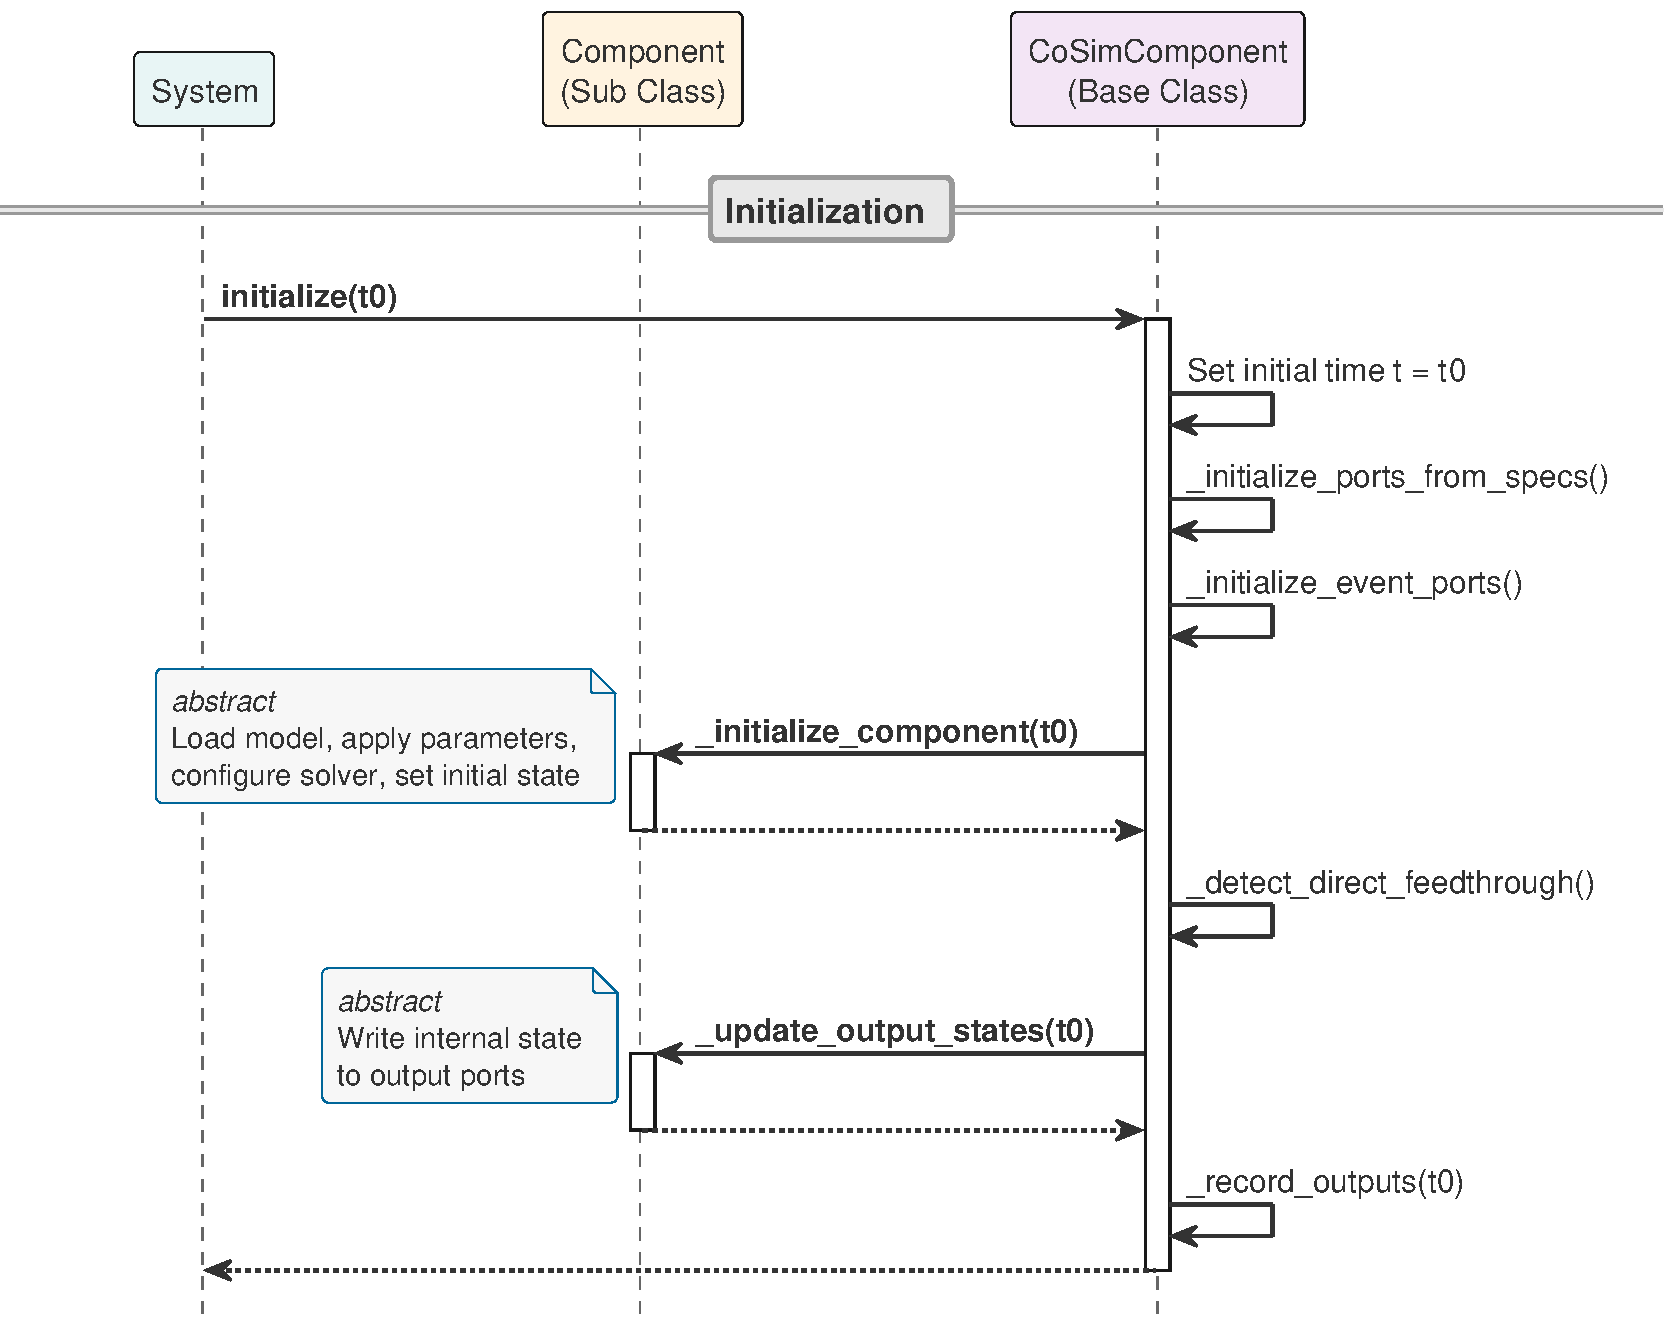
\includegraphics[width=0.8\linewidth]{diagrams/out/pdf/execution/CoSimComponent_Initialization.pdf}
  \caption{Delegation during component initialization. The template method
    \texttt{initialize()} performs the idempotency check, creates regular
    and event ports, delegates model-specific setup to
    \texttt{\_initialize\_component()}, detects direct feedthrough, publishes
    initial outputs through \texttt{\_update\_output\_states()}, and records
    the initial output values.}
  \label{fig:impl_comp_initialization}
\end{figure}

\paragraph{Simulation Step.}
Figure~\ref{fig:impl_comp_stepping} shows one macro step.
The master algorithm calls \texttt{do\_step(t,dt)}.
The template method delegates the numerical advancement to \texttt{\_do\_step\_internal()}.
After the subclass returns, the base class updates \texttt{t}, refreshes the output ports, and records the new output values.

\begin{figure}[btbp]
  \centering
  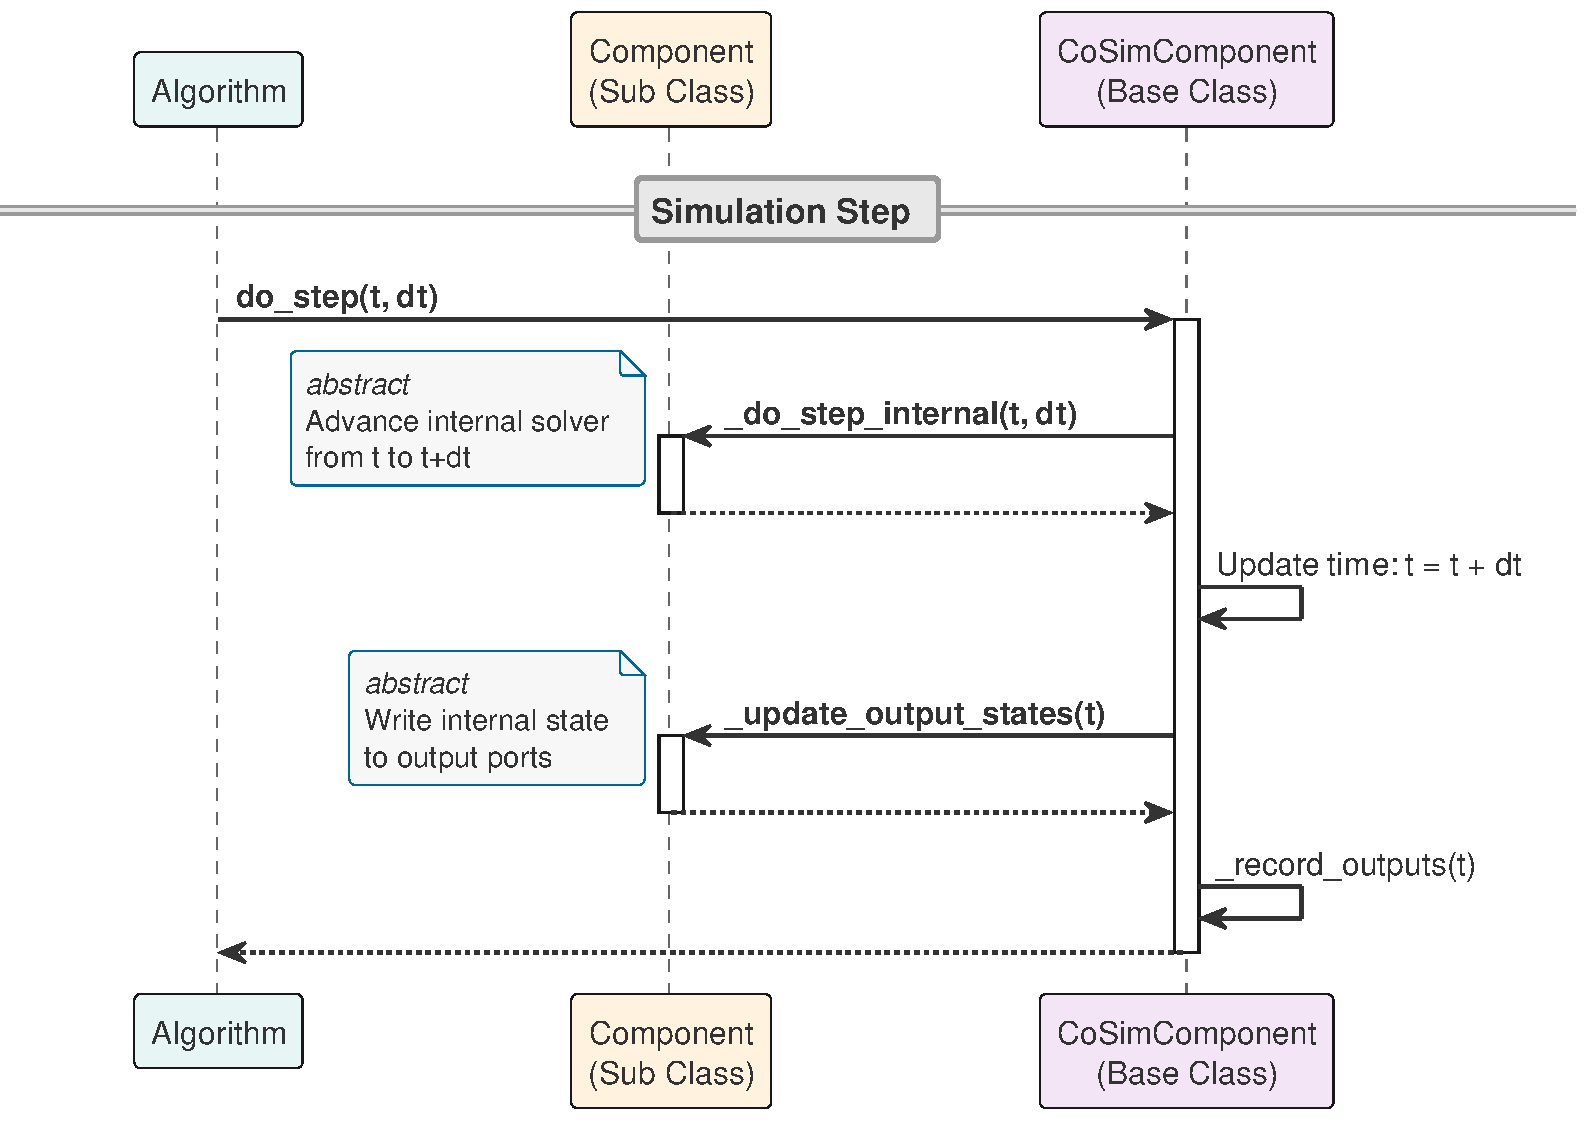
\includegraphics[width=0.8\linewidth]{diagrams/out/pdf/execution/CoSimComponent_Stepping.pdf}
  \caption{Delegation during a simulation step. The template method
    \texttt{do\_step()} delegates the computation to the primitive operation
    \texttt{\_do\_step\_internal()} and the output update to
    \texttt{\_update\_output\_states()}.}
  \label{fig:impl_comp_stepping}
\end{figure}

\paragraph{Event Handling.}
The template method \pyfn{handle\_event(event\_names,\,t)} is called by the hybrid algorithm at event times (Section~\ref{sec:impl_hybrid}).
It delegates the state update to the hook operation \pyfn{\_handle\_events\_internal()}, then calls \pyfn{\_update\_output\_states()} to refresh the output ports, and records the updated values in the component history.
Components that do not participate in hybrid simulation inherit an empty default for \pyfn{\_handle\_events\_internal()}, so the call is a no-op.

\paragraph{Reset and Cleanup.}
After the simulation loop, the hook operation \pyfn{reset()} supports component reuse.
It clears the simulation time, history buffer, and initialization flag, allowing the component to be re-initialized with \pyfn{initialize()} for a new run.
Subclasses extend the default implementation via \pyfn{super().reset()} to
additionally clear internal state.

%%%%%%%%%%%%%%%%%%%%%%%%%%%%%%%%%%%%%%%%%%%%%%%%%%%%%%
\subsection{Verification}

The verification of \texttt{CoSimComponent} targets framework-level invariants that are independent of any backend.
Lightweight mock subclasses, such as a pure-gain feedthrough component, a simple integrator, and minimal hybrid components, implement only the three primitive operations, keeping the tests focused on base-class behavior.

Table~\ref{tab:cosimcomp_verification} summarizes the verified base-class invariants.

\begin{table}[htbp]
  \centering
  \small
  \caption{Verification of the main \texttt{CoSimComponent} base-class invariants.}
  \label{tab:cosimcomp_verification}
  \begin{tabular}{p{5.8cm} p{8.2cm}}
    \toprule
    \textbf{Verified invariant} & \textbf{Expected outcome} \\
    \midrule
    Initialization lifecycle
      & \texttt{initialize()} creates port states, delegates model setup once, publishes initial outputs, records history, and remains idempotent \\
    \addlinespace
    Step lifecycle
      & \texttt{do\_step()} delegates numerical advancement, updates time, refreshes outputs, and records the stepped values \\
    \addlinespace
    Direct-feedthrough detection
      & Feedthrough components report algebraic input-output dependencies, while pure integrators report none \\
    \addlinespace
    Reset lifecycle
      & \texttt{reset()} clears time, history, and initialization state so that the component can be initialized again \\
    \addlinespace
    Event-port handling
      & Event output ports are created for registered event indicators before or after initialization \\
    \bottomrule
  \end{tabular}
\end{table}

The tests confirm that the base class enforces the component contract independently of any backend.
The template methods create port states, preserve lifecycle order, update output values, and record history consistently.
The feedthrough detector identifies algebraic dependencies for feedthrough components and leaves pure integrators without feedthrough.
Backend-specific hook behavior is verified in the corresponding wrapper sections because its correctness depends on the concrete model semantics.